% vim: set textwidth=78 autoindent:

%\subsection{MapServer Export Plugin}\label{sec:mapserver_export}
%
%You can use QGIS to ``compose'' your map by adding and arranging layers, 
%symbolizing them, customizing the colors and then create a map file 
%for MapServer. In order to use the MapServer Export plugin, you 
%must have Python >= 2.4 installed on your system and QGIS must have been 
%compiled with support for it. All binary packages include Python Support.
%
%The MapServer Export plugin in QGIS \CURRENT is a Python Plugin, that is 
%automatically loaded into the \filename{Plugin Manager} as a core plugin 
%(see Section~\ref{sec:core_plugins}).

\subsection{Extension d'exportation Mapserver}\label{sec:mapserver_export}

Vous pouvez utiliser QGIs pour ``composer'' votre carte en ajoutant et en arrangeant des couches, en modifiant leur repr\'esentation graphique, puis vous pouvez exporter le r\'esultat sous la forme d'un fichier .map \`a destination de MapServer. Pour utiliser cette extension, vous devez avoir Python >= 2.4 d'install\'e sur votre syst\`eme ainsi qu'une version de QGIs compil\'ee avec le support ad\'equat. Toutes les versions officielles disponibles offrent ce support de Python.

L'extension d'exportation Mapserver de QGIS \CURRENT est une extension python, qui est autmatiquement charg\'ee dans le \filename{Gestionnaire d'extension} comme l'une des extensions principales (voir Section~\ref{sec:core_plugins}).

%\subsubsection{Creating the Project File}
%
%The MapServer Export Plugin operates on a saved QGIS project file and 
%\textbf{not} on the current contents of the map canvas and legend. This 
%has been a source of confusion for a number of people. As described below, 
%before you start using the MapServer Export Plugin, you need to arrange 
%the raster and vector layers you want to use in MapServer and save this 
%status in a QGIS project file

\subsubsection{Cr\'eation du fichier de projet}

L'extension fonctionne sur une fichier de projet QGIS pr\'ec\'edemment enregistr\'e, et non \textbf{pas} sur le contenu actuel de la carte et de la l\'egende. C'est souvent une source de confusion pour beaucoups. Comme d\'ecrit ci-dessous, vous avez besoin de r\'earranger les couches vecteurs et rasters que vous voulez utiliser dans MapServer et enregistrer l'\'etat qui para\^it satisfaisant dans un fichier de projet QGIS.

%\begin{figure}[ht]
%\begin{center}
%  \caption{Arrange raster and vector layers for QGIS project file \nixcaption}
%  \label{fig:mapserver_export_qgs}\smallskip
%  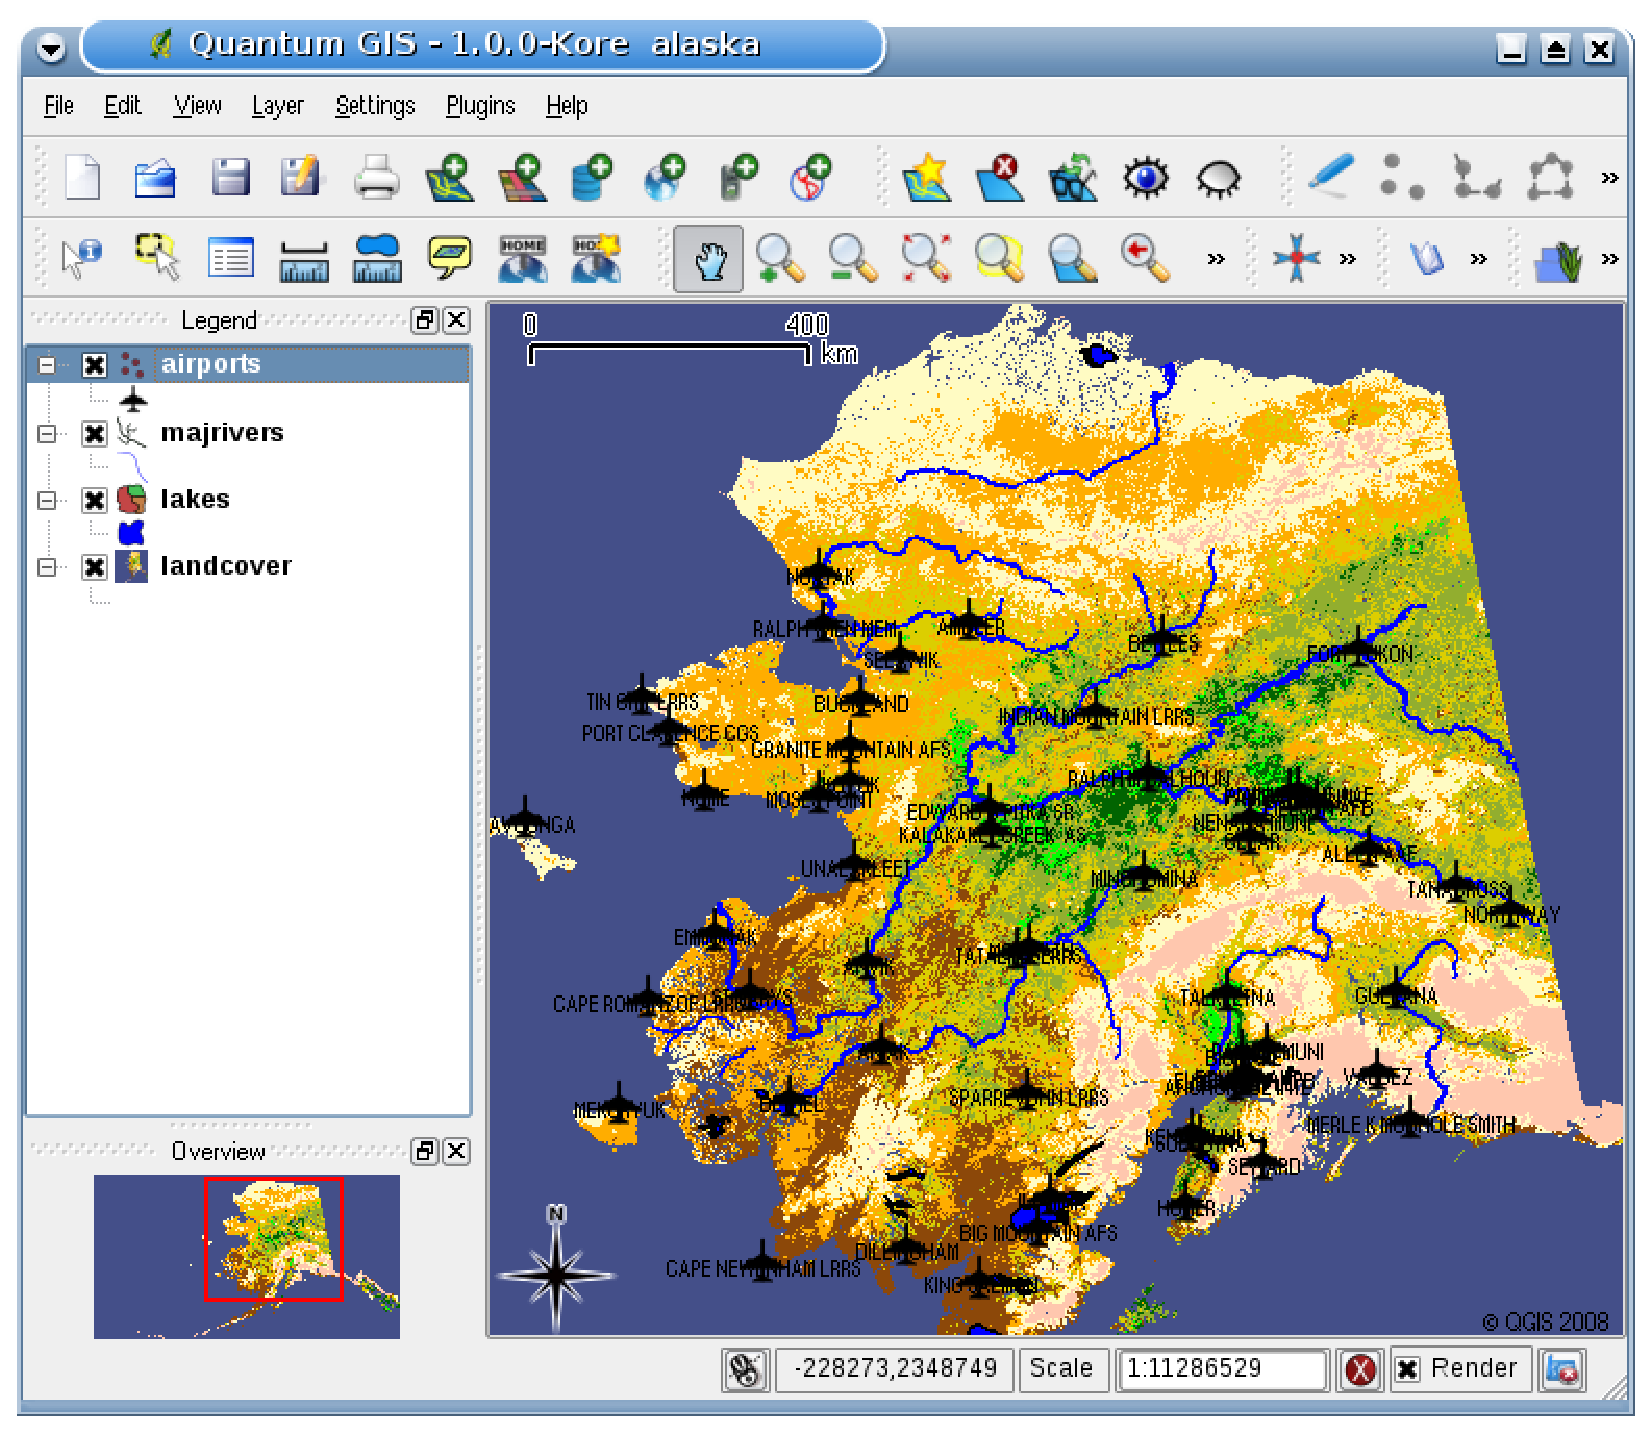
\includegraphics[clip=true, width=12cm]{mapserver_export_qgs}
%\end{center}
%\end{figure}

\begin{figure}[ht]
\begin{center}
  \caption{Arrangement des couches d'un fichier de projet QGIS \nixcaption}
  \label{fig:mapserver_export_qgs}\smallskip
  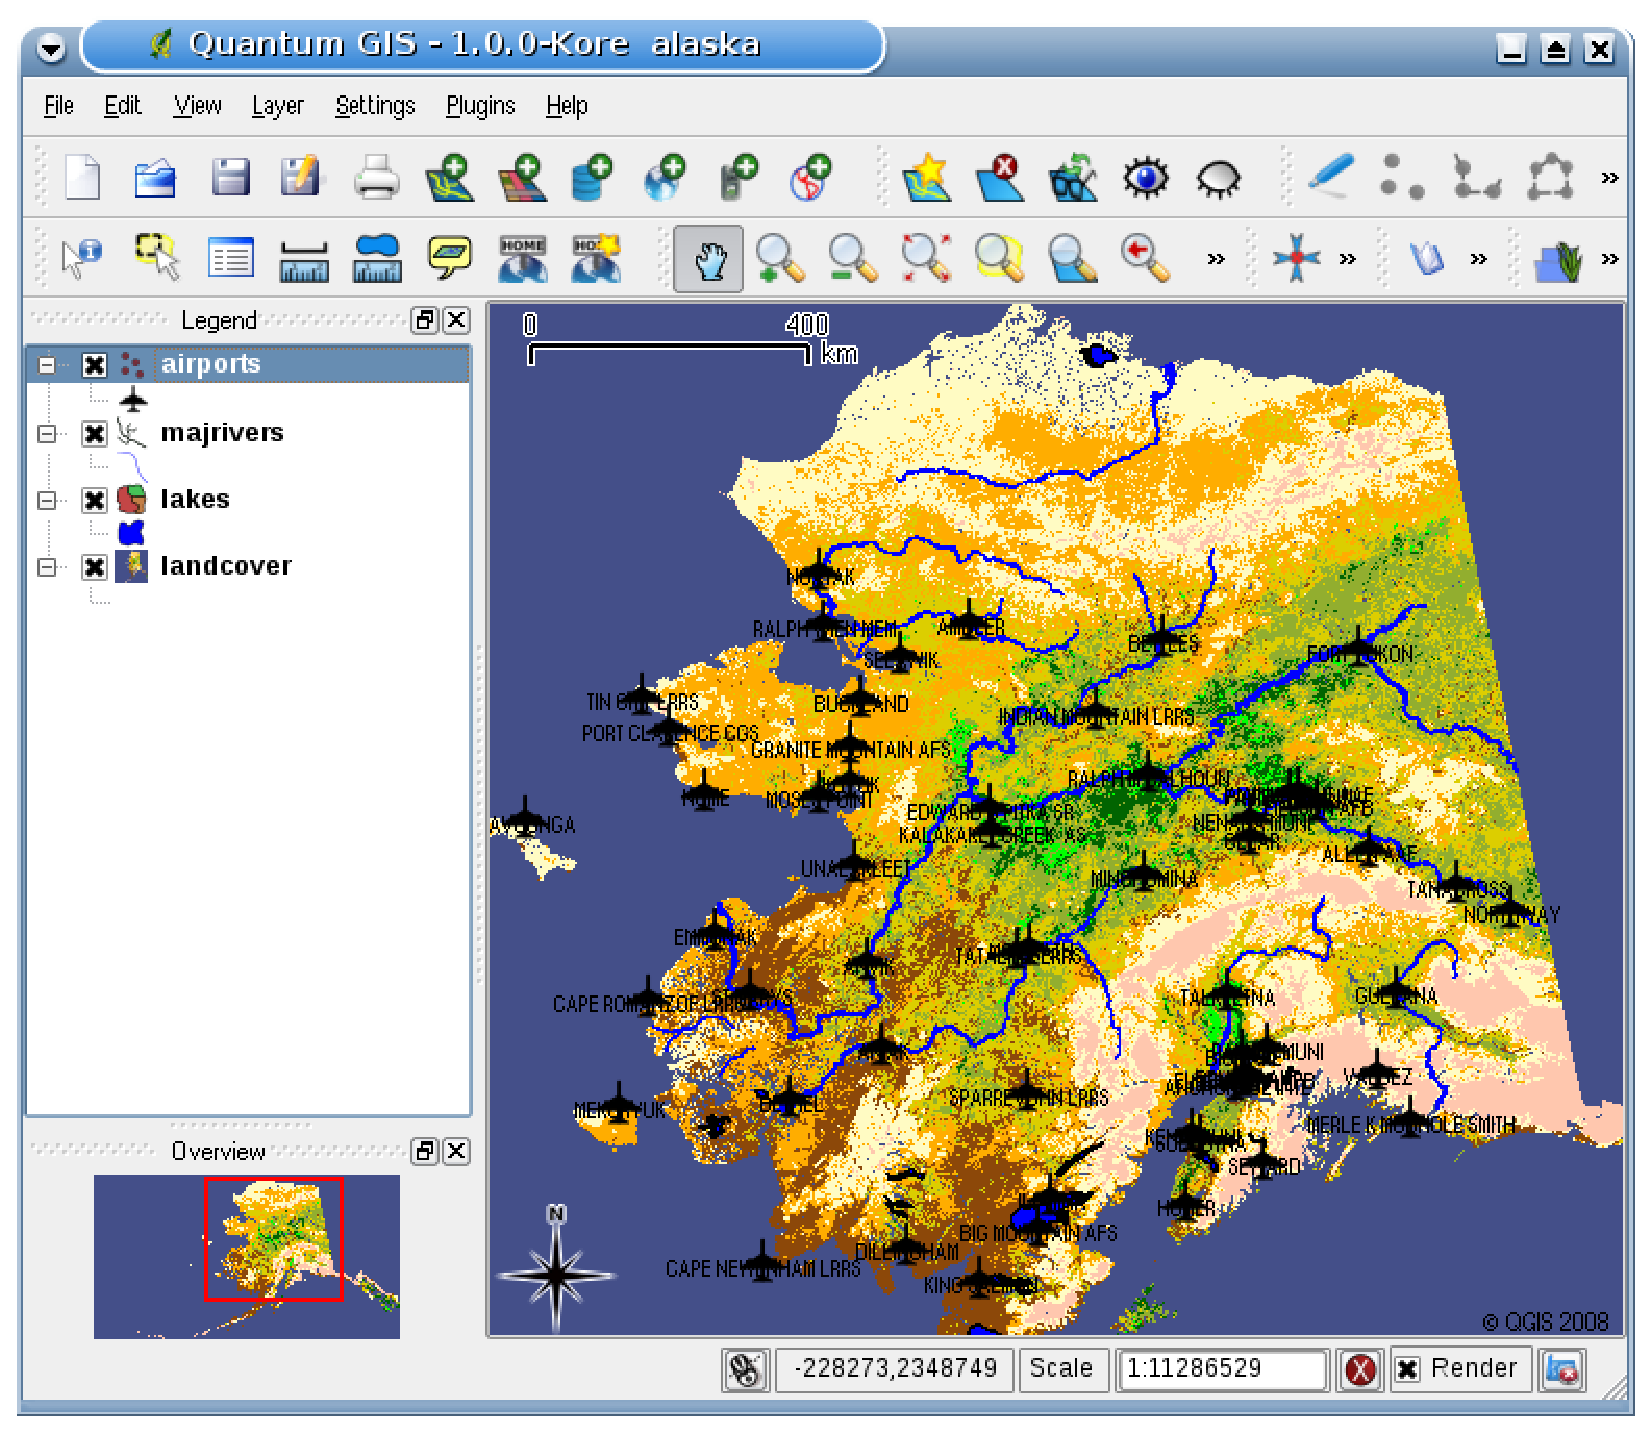
\includegraphics[clip=true, width=12cm]{mapserver_export_qgs}
\end{center}
\end{figure}

%In this example we show the four steps to get us to the point where we are 
%ready to create the MapServer map file. We use raster and vector files from 
%the QGIS sample dataset \ref{label_sampledata}.

Dans cet exemple est montr\'e les quatres \'etapes conduisant \`a la cr\'eation du fichier .map pour MapServer. Les fichiers vecteurs et rasters proviennent de l'\'echantillon de jeu de donn\'ees de Quantum GIS \ref{label_sampledata}.

%\begin{enumerate}
%\item Add the raster layer \filename{landcover.tif} clicking on the 
%\toolbtntwo{mActionAddRasterLayer}{Add Raster Layer} icon.
%\item Add the vector Shapefiles \filename{lakes.shp, majrivers.shp} and 
%\filename{airports.shp} from the QGIS sample dataset clicking on the 
%\toolbtntwo{mActionAddNonDbLayer}{Add Vector Layer} icon.
%\item Change the colors and symbolize the data as you like (see 
%Figure~\ref{fig:mapserver_export_qgs})
%\item Save a new project named \filename{mapserverproject.qgs} using 
%\mainmenuopt{File} > \dropmenuopttwo{mActionFileSave}{Save Project}.
%\end{enumerate} 

\begin{enumerate}
\item Ajoutez la couche raster \filename{landcover.tif} en cliquant sur l'ic\^one \toolbtntwo{mActionAddRasterLayer}{Ajouter une Couche Raster}.
\item Ajoutez la couche vecteur des shapefiles \filename{lakes.shp, majrivers.shp} et \filename{airports.shp} depuis le jeu de donn\'ees en cliquant sur l'ic\^one \toolbtntwo{mActionAddNonDbLayer}{Ajouter une couche Vecteur}.
\item Changer les couleurs et les symboles des donn\'ees (voir Figure~\ref{fig:mapserver_export_qgs})
\item Enregistrez dans un nouveau fichier de projet nomm\'e \filename{mapserverproject.qgs} en utilisant \mainmenuopt{File} > \dropmenuopttwo{mActionFileSave}{Enregistrer le projet}.
\end{enumerate} 

%\subsubsection{Creating the Map File}
%
%The tool \filename{msexport} to export a QGIS project file to a MapServer map 
%file is installed in your QGIS binary directory and can be used independently of QGIS. 
%From QGIS you need to load the MapServer Export Plugin first with the Plugin Manager. 
%Click \mainmenuopt{Plugins} > \dropmenuopt{Manage Plugins...} to open the Plugin Manager, 
%choose MapServer export Plugin and click \button{OK}. Now start the 
%\toolbtntwo{mapserver_export}{MapServer Export} dialog (see 
%Figure~\ref{fig:mapserver_export_dialog}) clicking the icon in the toolbar menu.

\subsubsection{Cr\'eation du fichier .map}

L'outil \filename{msexport} d'exportation se situ dans votre r\'epertoiret d'installation de QGIS et peut \^etre utilis\'e ind\'ependamment de QGIS. Pour l'utiliser \`a partir du logiciel vous devez charger l'extension en utilisant le Gestionaire d'extension. Cliquez sur \mainmenuopt{Plugins} > \dropmenuopt{Gestionnaire d'extension} pour l'ouvrir, s\'electionnez l'extension d'exportation vers MapServer et faites \button{OK}. Maintenant lancez le dialogue \toolbtntwo{mapserver_export}{Exporter vers MapServer} (voir Figure~\ref{fig:mapserver_export_dialog}) en cliquant sur l'ic\^one dans la barre de menu.

%\begin{figure}[ht]
%\begin{center}
%  \caption{Export to MapServer Dialog \nixcaption}
%  \label{fig:mapserver_export_dialog}\smallskip
%  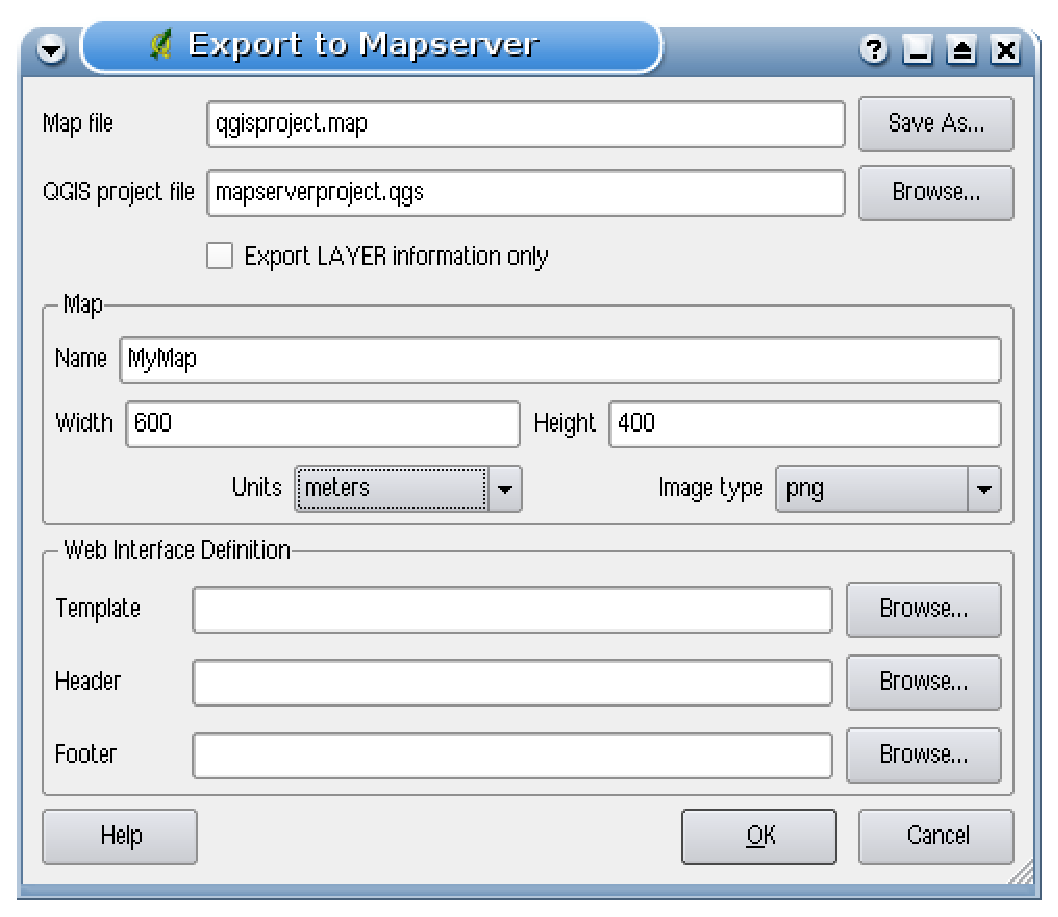
\includegraphics[clip=true, width=10cm]{mapserver_export_dialog}
%\end{center}
%\end{figure}

\begin{figure}[ht]
\begin{center}
  \caption{Dialogue d'exportation vers MapServer \nixcaption}
  \label{fig:mapserver_export_dialog}\smallskip
  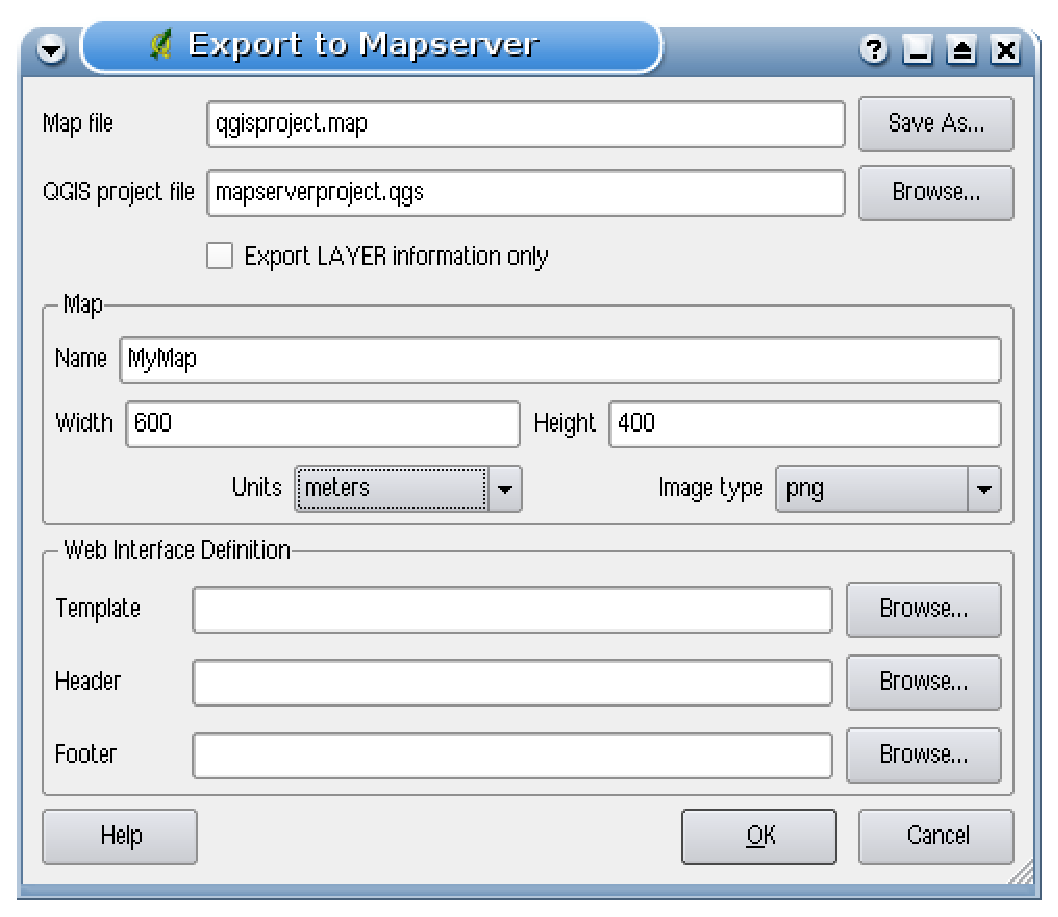
\includegraphics[clip=true, width=10cm]{mapserver_export_dialog}
\end{center}
\end{figure}

%\begin{description}
%\item [Map file] \mbox{}\\
%Enter the name for the map file to be created. You can use the button at the 
%right to browse for the directory where you want the map file created. 
%\item [Qgis project file] \mbox{}\\
%Enter the full path to the QGIS project file (.qgs) you want to export. You can 
%use the button at the right to browse for the QGIS project file.
%\item [Map Name] \mbox{}\\
%A name for the map. This name is prefixed to all images generated by the mapserver.
%\item [Map Width] \mbox{}\\
%Width of the output image in pixels.
%\item [Map Height] \mbox{}\\
%Height of the output image in pixels.
%\item [Map Units] \mbox{}\\
%Units of measure used for output
%\item [Image type] \mbox{}\\
%Format for the output image generated by MapServer
%\item [Web Template] \mbox{}\\
%Full path to the MapServer template file to be used with the map file
%\item [Web Header] \mbox{}\\
%Full path to the MapServer header file to be used with the map file
%\item [Web Footer] \mbox{}\\
%Full path to the MapServer footer file to be used with the map file
%\end{description}

\begin{description}
\item [Fichier .map] \mbox{}\\
Saissez le chemin complet du fichier .map que vous voulez exporter. Vous pouvez utiliser le bouton sur la droite pour parcourir votre syst\`eme.
\item [Fichier projet Qgis] \mbox{}\\
Saissez le chemin complet du fichier projet (.qgs) que vous voulez exporter. Vous pouvez utiliser le bouton sur la droite pour parcourir votre syst\`eme.
\item [Nom de la carte] \mbox{}\\
Un nom pour la carte. Ce nom pr\'efixera toutes les images cr\'e\'ees par le serveur.
\item [Largeur de la carte] \mbox{}\\
Largeur en pixels de l'image g\'en\'er\'ee.
\item [Hauteur de la carte] \mbox{}\\
hauteur en pixels de l'image g\'en\'er\'ee.
\item [Unit\'ees de la carte] \mbox{}\\
Unit\'ees de mesure utilis\'ees
\item [Type d'image] \mbox{}\\
Format de l'image g\'en\'er\'ee par MapServer
\item [Web Template] \mbox{}\\
Chemin complet vers le fichier MapServer template \`a utiliser
\item [Web en-t\^ete] \mbox{}\\
Chemin complet vers le fichier d'en-t\^ete de MapServer \`a utiliserMapServer
\item [Web bas de page] \mbox{}\\
Chemin complet vers le fichier de bas de page MapServer \`a utiliser
\end{description}

Seulement le \filename{fichier .map} et le \filename{fichier de projet QGIS} sont requis pour cr\'eer un fichier .map, vous risquez cependant d'obtenir un fichier inutilisable ce que vous d\'esirez en faire. Bien que QGIS soit bon pour cr\'eer les fichiers .map, votre projet n\'ecessite peut-\^etre des adaptions pour obtenir le r\'esultat escompt\'e. Cr\'eons un fichier .map en utilisant le projet \filename{mapserverproject.qgs} que nous avons cr\'e\'e (voir Figure~\reffig:mapserver_export_dialog}):

%Only the \filename{Map file} and \filename{QGIS project file} inputs are 
%required to create a map file, however you may end up with a non-functional 
%map file, depending on your intended use. Although QGIS is good at creating 
%a map file from your project file, it may require some tweaking to get the 
%results you want. But let's create a map file using the project file 
%\filename{mapserverproject.qgs} we just created 
%(see Figure~\ref{fig:mapserver_export_dialog}):

%\begin{enumerate}
%  \item Open the MapServer Export Plugin clicking the 
%  \toolbtntwo{mapserver_export}{MapServer Export} icon.
%  \item Enter the name \filename{qgisproject.map} for your new map file.
%  \item Browse and find the QGIS project file \filename{mapserverproject.qgs} 
%  you just saved.
%  \item Enter a name \filename{MyMap} for the map.
%  \item Enter \filename{600} for the width and \filename{400} for the height.
%  \item Our layers are in meters so we change the units to meters.
%  \item Choose ``png'' for the image type.
%  \item Click \button{OK} to generate the new map file \filename{qgisproject.map}. 
%  QGIS displays the success of your efforts.
%\end{enumerate}

\begin{enumerate}
  \item Ouvrez l'extension en cliquant sur l'ic\^one \toolbtntwo{mapserver_export}{Exporter vers }.
  \item Entrez le nom \filename{qgisproject.map} pour votre nouveau fichier .map.
  \item S\'electionnez le projet QGIS \filename{mapserverproject.qgs} que vous venez d'enregistrer.
  \item Entrez un nom \filename{MaCarte} pour la carte.
  \item Entrez \filename{600} pour la largeur et \filename{400} pour la hauteur.
  \item Nos couches sont en m\`etres, l'unit\'e de mesure sera donc le m\`etre.
  \item Choisissez ``png'' pour le type d'image.
  \item Cliquez sur \button{OK} pour g\'en\'erer le ouveau fichier \filename{qgisproject.map}. 
  QGIS affiche le r\'esultat de vos efforts.
\end{enumerate}

%You can view the map file in an text editor or visualizer. If you
%take a look, you'll notice that the export tool adds the metadata needed
%to enable our map file for WMS. 

Vous pouvez visualiser le fichier .map dans un \'editeur de texte. Si vous le faite, vous remarquerez que l'outil d'exportation ajoute les m\'etadonn\'ees n\'ecessaires \`a l'utilisation du protocole WMS.

%\subsubsection{Testing the Map File}
%
%We can now test our work using the \filename{shp2img} tool to create an image
%from the map file. The \filename{shp2img} utility is part of MapServer and FWTools. 
%To create an image from our map:

\subsubsection{Essai du fichier .map}

We can now test our work using the \Nus povuons maintenant tester notre travail en utilisant l'outil \filename{shp2img} pour cr\'eer une image tir\'ee du fichier .map. Cet outil est pr\'esent dans MapServer et FWTools. 
Pour cr\'eer une image :

%\begin{itemize}
%\item Open a terminal window
%\item If you didn't save your map file in your home directory, change to
%  the folder where you saved it
%\item Run \filename{shp2img -m qgisproject.map -o mapserver\_test.png} and 
%  display the image 
%\end{itemize}
% 
%This creates a PNG with all the layers included in the QGIS project file. 
%In addition, the extent of the PNG will be the same as when we saved the 
%project. As you can see in Figure~\ref{fig:mapserver_export_test}, all 
%inforamtion except the airport symbols are included.

\begin{itemize}
\item Ouvrez une console de commande
\item Si vous n'avez pas sauvegard\'e votre fichier dans votre r\'epertoire personnel, d\'eplacer vers le bon dossier
\item Lancez \filename{shp2img -m qgisproject.map -o mapserver\_test.png} et affichez l'image
\end{itemize}
 
Une image PNG est cr\'e\'ee avec toutes les couches du projet QGIS. En compl\'ement, l'\'etendue du PNG sera la m\^eme que celle du projet. Comme vous le voyez sur la figure~\ref{fig:mapserver_export_test}, toutes les informations, \`a l'exception des symboles des a\'eroports, sont inclues.

%\begin{figure}[ht]
%\begin{center}
%  \caption{Test PNG created by shp2img with all MapServer Export layers \nixcaption}
%  \label{fig:mapserver_export_test}\smallskip
%  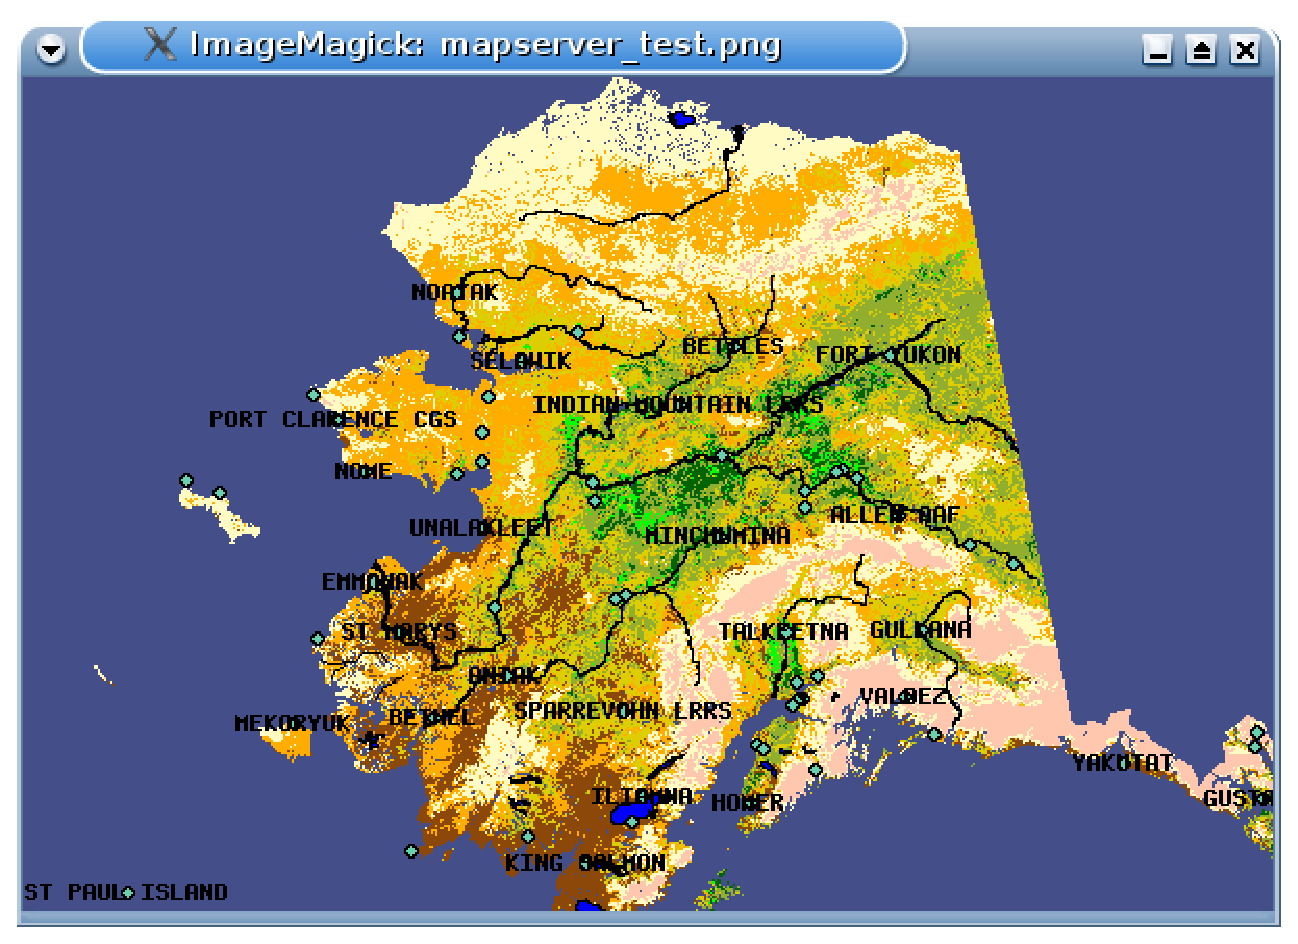
\includegraphics[clip=true, width=12cm]{mapserver_export_test}
%\end{center}
%\end{figure}
%
%If you plan to use the map file to serve WMS requests, you probably don't
%have to tweak anything. If you plan to use it with a mapping template or a
%custom interface, you may have a bit of manual work to do. To see how easy
%it is to go from QGIS to serving maps on the web, take a look at
%Christopher Schmidt's 5 minute flash video. He used QGIS version 0.8, but it 
%is still useful.
%\footnote{\url{http://openlayers.org/presentations/mappingyourdata/}}

\begin{figure}[ht]
\begin{center}
  \caption{Image PNG cr\'e\'ee par shp2img \nixcaption}
  \label{fig:mapserver_export_test}\smallskip
  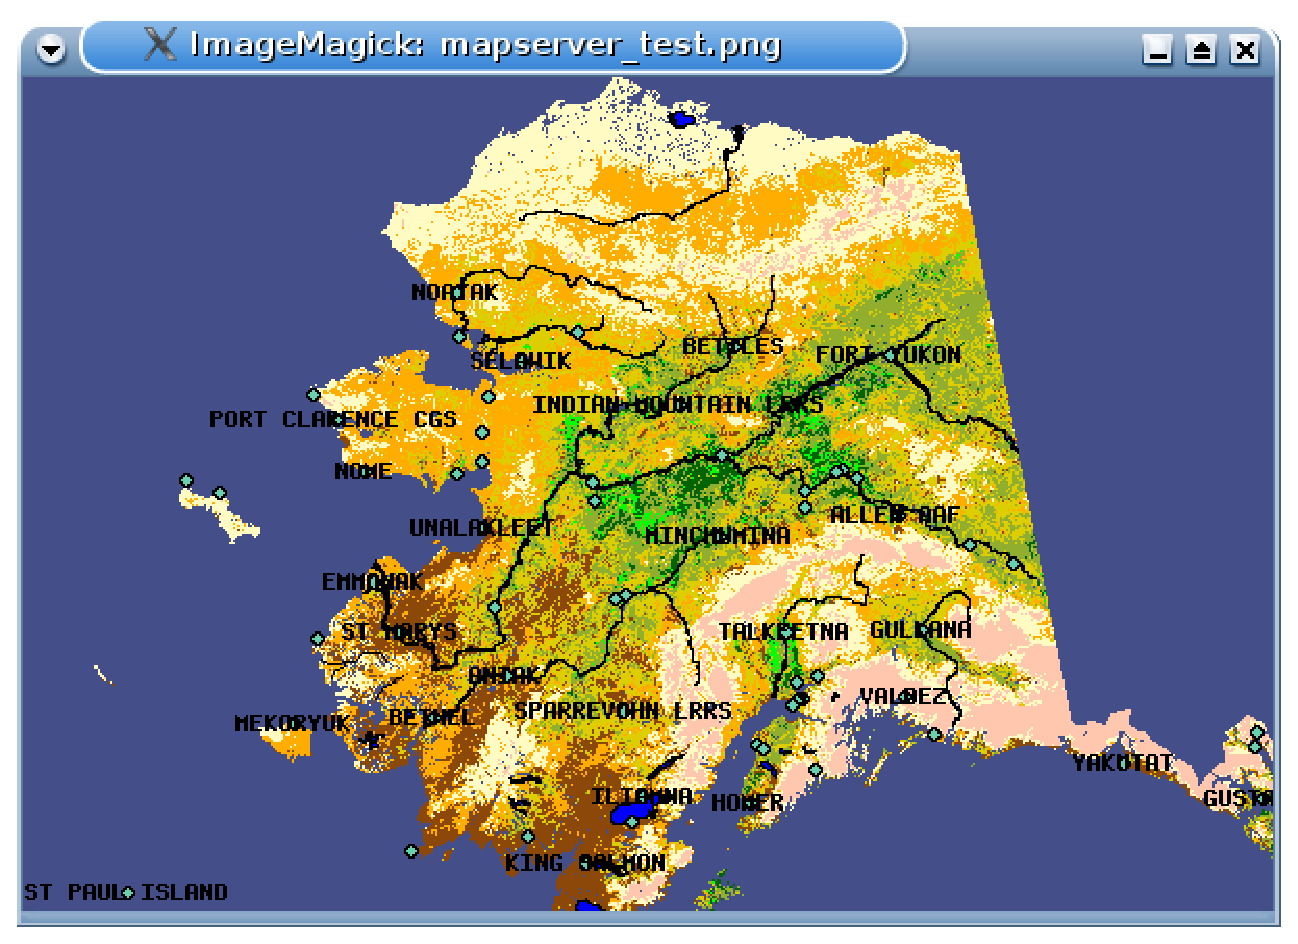
\includegraphics[clip=true, width=12cm]{mapserver_export_test}
\end{center}
\end{figure}

Si vous comptez utiliser ce fichier .map pour fournir un service WMS, vous n'aurez probablement rien d'autres \`a modifier. Par contre si vous comptez l'utiliser comme mod\`ele ou dans une interface personnalis\'ee vous aurez un peu plus de travaux manuels \`a effectuer. Jetez un oeil sur cette vid\'eo de Christopher Schmidt, il a utilis\'e la version 0.8 de QGIS version 0.8 mais cela reste utile.
\footnote{\url{http://openlayers.org/presentations/mappingyourdata/}}
